\documentclass[10pt,notheorems,xcolor=pdftex,dvipsnames,table]{beamer}
\usepackage[utf8]{inputenc}
\definecolor{light-gray}{gray}{0.95}
\setbeamercolor{background canvas}{bg=light-gray}
\linespread{1.2}
\usepackage[absolute,overlay]{textpos}
\usepackage{graphicx}
\usepackage{cancel}
\usefonttheme{serif}
\usepackage[T1]{fontenc}
\usepackage[english]{babel}
\usepackage{amsmath}
\usepackage{amsfonts}
\usepackage{amsthm}
%\usepackage[usenames,dvipsnames]{xcolor}
\usepackage{amssymb}
\usepackage{hyperref}
\usepackage{xr}
\usepackage[all]{xy}
\usepackage{tikz-cd}
\usepackage{hyperref}
\usepackage{filecontents}
\usepackage[english, status=draft]{fixme}
\fxusetheme{color}
\usepackage{cleveref} 
\usepackage[backgroundcolor=cyan]{todonotes}
\usepackage{wallpaper}
\usepackage{faktor}
\usepackage{float}
\usepackage{tikz}
\usetikzlibrary{calc, 3d,automata,positioning,decorations.pathreplacing}
\usepackage{listings}
\usepackage{array}

\usepackage{calligra}


\renewcommand{\{}{\left\lbrace}
\renewcommand{\}}{\right\rbrace}
\newcommand{\C}{\mathbb{C}}
\newcommand{\R}{\mathbb{R}}
\newcommand{\Z}{\mathbb{Z}}
\newcommand{\Q}{\mathbb{Q}}
\newcommand{\N}{\mathbb{N}}
\newcommand{\Gal}{\mathrm{Gal}}
\newcommand{\Aut}{\mathrm{Aut}}
\newcommand{\IN}{\mathrm{in}_{\leq}}
\newcommand{\lex}{\leq_{\mathrm{lex}}}
\newcommand{\lcm}{\mathrm{lcm}}
\newcommand{\wdots}[2]{ #1, \ldots ,#2 }
\renewcommand{\P}{\{ \wdots{p_1}{p_m} \}}
\newcommand{\K}{K[ \wdots{x_1}{x_n} ]}
\newcommand{\I}{\langle \wdots{p_1}{p_m}  \rangle}


\newtheoremstyle{break}
	{\topsep}{\topsep}
	{\bfseries}{}
	{\newline}{}
\theoremstyle{break}
\newtheorem{theorem}{Theorem}
\newtheorem{lemma}{Lemma}
\newtheorem{proposition}{Proposition}
\newtheorem{corollary}{Corollary}
\newtheorem{definition}{Definition}
\newtheoremstyle{Break}
	{\topsep}{\topsep}
	{}{}
	{\bfseries}{}
	{\newline}{}
\theoremstyle{Break}
\newtheorem{example}{Example}


\newcommand{\divides}{\bigm|}
\newcommand{\ndivides}{%
  \mathrel{\mkern.5mu % small adjustment
    % superimpose \nmid to \big|
    \ooalign{\hidewidth$\big|$\hidewidth\cr$\nmid$\cr}%
  }%
}


\begin{document}

\begin{frame}
	\frametitle{ \vspace*{1.5cm}
		\begin{center} 
			\Huge{Integer Programming Models in Graph Coloring} \linebreak \linebreak
			\normalsize{Bachelor defence by Christian Buchter \\
			June 16th 2017}
		\end{center}}
\end{frame}


\begin{frame}[t]
	\frametitle{ 
		\LARGE{Presentation plan}}
			\begin{enumerate}
				\item<1-> Motivation and background
					\tikz[remember picture] \node[coordinate,xshift=0.3cm, yshift=0.2cm] (n1) {};
				\item<1-> Linear programming
				\item<1-> Graph colouring			
				\item<1-> Integer programming
				\item<1-> IP colouring formulations
				\item<1-> Lego graphs
				\item<1-> Exciting results
				\item<1-> Short summary
					\tikz[remember picture] \node[coordinate, xshift=2.18cm, yshift=-0.1cm] (n2) {};
				\item<3->  Questions
			\end{enumerate}
				\visible<2->{
					\begin{tikzpicture}[overlay,remember picture]
						\draw[thick,decorate,decoration={brace,amplitude=7pt}]
				    	(n1) -- (n2) node[midway, right=10pt] {25 min.};
					\end{tikzpicture} 		} 
\end{frame}




	
\begin{frame}[t]
\frametitle{
		\LARGE{1. Motivation and background}}
			\visible<2->{ Solving a hard combinatorial problem in an efficient way. }
			\centering
				\visible<3->{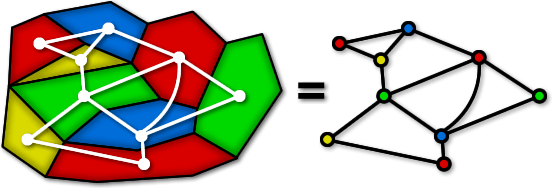
\includegraphics[scale=0.35]{fourcolour.png} }
			\begin{textblock*}{3cm}(1cm,4.5cm)
				\visible<4->{
				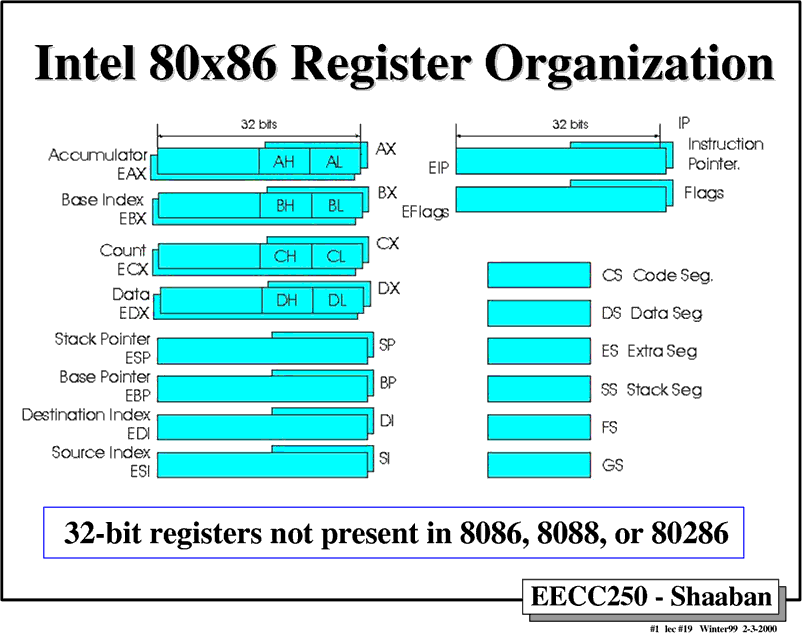
\includegraphics[scale=0.2]{IntelRegisters.png}
				} 
			\end{textblock*}
			\begin{textblock*}{3cm}(7cm,5.5cm)
				\visible<5->{
				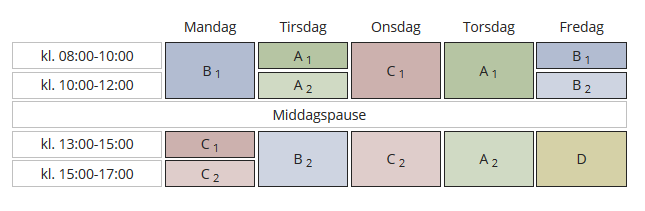
\includegraphics[scale=0.4]{skemagruppe.PNG}
				} 
			\end{textblock*}
\end{frame}

\begin{frame}[t]
\frametitle{
		\LARGE{1. Motivation and background}}
			\centering
				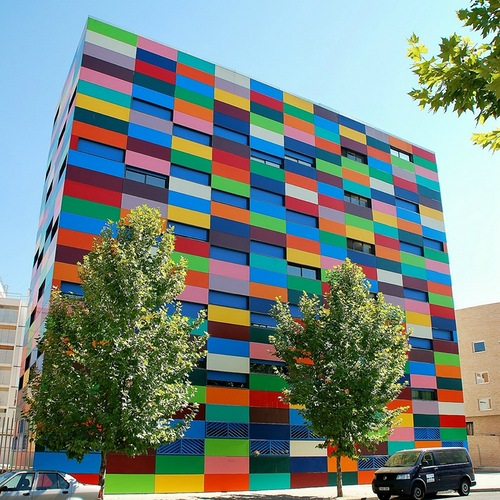
\includegraphics[scale=1.8]{legoBuilding.jpg}
\end{frame}



\begin{frame}[t]
\frametitle{
		\LARGE{2. Linear programming}}
		\visible<2->{
		Optimizing an objective subject to constraints
		}
			\visible<3->{
					\begin{align*}
\begin{array}{ll@{}ll}
\text{min/max} &z(x_1,...,x_n)&\\
\text{s.t.} &g_1(x_1,...,x_n) \textbf{ ordRel } b_1,&\\
&\vdots&\\
&g_m(x_1,...,x_n) \textbf{ ordRel } b_m&\\
&\text{where each \textbf{ordRel} can be }\leq,\geq \text{ or } =&
\end{array}
					\end{align*}
			}
			\visible<4->{ $x_1,...,x_n \in \R$\\}
			\visible<5->{These problems are easy and can be solved in polynomial time.}
			\visible<6->{
			\begin{example}
			\vspace*{-1.1cm}
			\begin{align}
\begin{array}{ll@{}ll}
\text{min} &5x_1+x_2+2x_3&\\
\text{s.t.} &3x_1+x_2+\frac{1}{2}x_3 \geq 6,&\\
&3x_1+2x_2+4x_3 \geq 15,&\\
&2x_1+x_3 \geq 5,&\\
&x_1+4x_2 \geq 7,&\\
&x_1,x_2,x_3 \geq 0&\\
\end{array}
\end{align}
			\end{example}
			}
\end{frame}


\begin{frame}[t]
\frametitle{
		\LARGE{2. Linear programming}}
		The feasible set and optimal solutions
		\visible<2->{
			\begin{figure}[H]
\centering
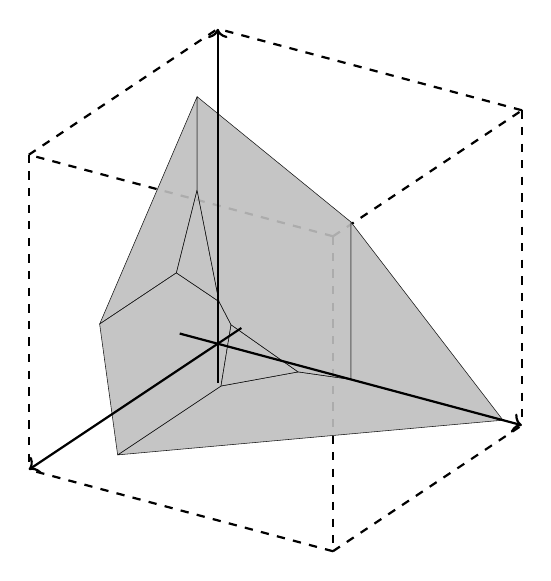
\begin{tikzpicture}[x  = {(0.9659cm,-0.25882cm)},
                    y  = {(-0.6cm,-0.4cm)},
                    z  = {(0cm,1cm)},
                    scale = 0.25,
                    color = {black}]
% style of faces
\tikzset{facestyle/.style={fill=black,draw=black,very thin,line join=round}}
% axis 
% coordinates
%x1>0
\coordinate (C1) at (0, 7/4, 53/4);
\coordinate (C2) at (0, 10, 5);
\coordinate (C3) at (0, 7/4, 17/2);
\coordinate (C4) at (0, 7/2, 5);
%x_2>0
\coordinate (C5) at (15, 0, 0);
\coordinate (C6) at (7, 0, 0);
\coordinate (C7) at (7, 0, 8);
%x3>0
%(C5) (C6)
\coordinate (C8) at (5/2, 25/2, 0);
\coordinate (C9) at (5/2, 15/4, 0);
\coordinate (C10) at (23/5, 3/5, 0);
%intersections
\coordinate (C11) at (17/11, 15/11, 21/11);
\coordinate (C12) at (1, 3/2, 3);%optimal
%objective plane
\coordinate (O1) at (10, 0, 0);
\coordinate (O2) at (10, 0, 10);
\coordinate (O4) at (0, 10, 0);
\coordinate (O3) at (0, 10, 10);

%box
\draw [black, dashed, thick] (16,16,0) -- (16,0,0);
\draw [black, dashed, thick] (16,16,0) -- (0,16,0);
\draw [black, dashed, thick] (16,0,16) -- (16,0,0);
\draw [black, dashed, thick] (16,0,16) -- (0,0,16);
\draw [black, dashed, thick] (0,16,16) -- (0,16,0);
\draw [black, dashed, thick] (0,16,16) -- (0,0,16);
\draw [black, dashed, thick] (16,16,16) -- (0,16,16);
\draw [black, dashed, thick] (16,16,16) -- (16,0,16);
\draw [black, dashed, thick] (16,16,16) -- (16,16,0);

%fill polyhedron-
%C1
\draw[fill=lightgray,draw=black,opacity=.9,very thin,line join=round]
 (C1) --
 (C2) --
 (C4) -- 
 (C3) -- cycle ;
 %C3
\draw[fill=lightgray,draw=black,opacity=.9,very thin,line join=round]
 (C5) --
 (C6) --
 (C7) --cycle ;
 %C4
\draw[fill=lightgray,draw=black,opacity=.9,very thin,line join=round]
  (C5) --
  (C6) --
  (C10)--
  (C9)--
  (C8)-- cycle ;
\draw[fill=lightgray,draw=black,opacity=.9,very thin,line join=round]
  (C8) --
  (C9) --
  (C11)--
  (C12)--
  (C4)--
  (C2)-- cycle ;
\draw[fill=lightgray,draw=black,opacity=.9,very thin,line join=round]
  (C10) --
  (C9) --
  (C11)-- cycle ;
\draw[fill=lightgray,draw=black,opacity=.9,very thin,line join=round]
  (C12) --
  (C3) --
  (C4)-- cycle ;
\draw[fill=lightgray,draw=black,opacity=.9,very thin,line join=round]
  (C7) --
  (C6) --
  (C10)--
  (C11)--
  (C12)--
  (C3)-- 
  (C1)--cycle ;
  
  \iffalse
%objective:
\draw[fill=green,draw=green,opacity=.5,very thin,line join=round]
(O1)--
(O2)--
(O3)--
(O4)--cycle;

\draw[fill=blue] (C12) circle (0.5em)
	    node[above right] {$(x_1=1,x_2=1.5,x_3=3)$};
%C2
%\draw[fill=gray,draw=red,opacity=.8,very thin,line join=round]
% (A232) --
% (A242) --
% (A231) --
% (A241) --
% (A122) --cycle ;
\draw [blue, arrows = ->] (5,3,4) -- (3,2.5,2.5);
\draw [blue, arrows = ->] (-1,2,4) -- (-3,1.5,2.5);
\fi
%extreme points
\draw [black, thick, arrows = ->] (0,0,-2) -- (0,0,16);
\draw [black, thick, arrows = ->] (0,-2,0) -- (0,16,0);
\draw [black, thick, arrows = ->] (-2,0,0) -- (16,0,0);
\end{tikzpicture}
\caption{A graphical repressentation of an LP.}
\end{figure}
}
\end{frame}


\begin{frame}[t]
\frametitle{
		\LARGE{2. Linear programming}}
		The feasible set and optimal solutions
			\begin{figure}[H]
\centering
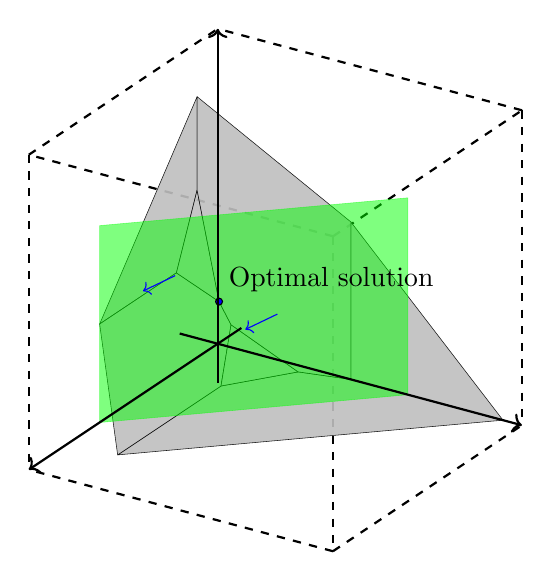
\begin{tikzpicture}[x  = {(0.9659cm,-0.25882cm)},
                    y  = {(-0.6cm,-0.4cm)},
                    z  = {(0cm,1cm)},
                    scale = 0.25,
                    color = {black}]
% style of faces
\tikzset{facestyle/.style={fill=black,draw=black,very thin,line join=round}}
% axis 
% coordinates
%x1>0
\coordinate (C1) at (0, 7/4, 53/4);
\coordinate (C2) at (0, 10, 5);
\coordinate (C3) at (0, 7/4, 17/2);
\coordinate (C4) at (0, 7/2, 5);
%x_2>0
\coordinate (C5) at (15, 0, 0);
\coordinate (C6) at (7, 0, 0);
\coordinate (C7) at (7, 0, 8);
%x3>0
%(C5) (C6)
\coordinate (C8) at (5/2, 25/2, 0);
\coordinate (C9) at (5/2, 15/4, 0);
\coordinate (C10) at (23/5, 3/5, 0);
%intersections
\coordinate (C11) at (17/11, 15/11, 21/11);
\coordinate (C12) at (1, 3/2, 3);%optimal
%objective plane
\coordinate (O1) at (10, 0, 0);
\coordinate (O2) at (10, 0, 10);
\coordinate (O4) at (0, 10, 0);
\coordinate (O3) at (0, 10, 10);

%box
\draw [black, dashed, thick] (16,16,0) -- (16,0,0);
\draw [black, dashed, thick] (16,16,0) -- (0,16,0);
\draw [black, dashed, thick] (16,0,16) -- (16,0,0);
\draw [black, dashed, thick] (16,0,16) -- (0,0,16);
\draw [black, dashed, thick] (0,16,16) -- (0,16,0);
\draw [black, dashed, thick] (0,16,16) -- (0,0,16);
\draw [black, dashed, thick] (16,16,16) -- (0,16,16);
\draw [black, dashed, thick] (16,16,16) -- (16,0,16);
\draw [black, dashed, thick] (16,16,16) -- (16,16,0);

%fill polyhedron-
%C1
\draw[fill=lightgray,draw=black,opacity=.9,very thin,line join=round]
 (C1) --
 (C2) --
 (C4) -- 
 (C3) -- cycle ;
 %C3
\draw[fill=lightgray,draw=black,opacity=.9,very thin,line join=round]
 (C5) --
 (C6) --
 (C7) --cycle ;
 %C4
\draw[fill=lightgray,draw=black,opacity=.9,very thin,line join=round]
  (C5) --
  (C6) --
  (C10)--
  (C9)--
  (C8)-- cycle ;
\draw[fill=lightgray,draw=black,opacity=.9,very thin,line join=round]
  (C8) --
  (C9) --
  (C11)--
  (C12)--
  (C4)--
  (C2)-- cycle ;
\draw[fill=lightgray,draw=black,opacity=.9,very thin,line join=round]
  (C10) --
  (C9) --
  (C11)-- cycle ;
\draw[fill=lightgray,draw=black,opacity=.9,very thin,line join=round]
  (C12) --
  (C3) --
  (C4)-- cycle ;
\draw[fill=lightgray,draw=black,opacity=.9,very thin,line join=round]
  (C7) --
  (C6) --
  (C10)--
  (C11)--
  (C12)--
  (C3)-- 
  (C1)--cycle ;
  
%objective:
\draw[fill=green,draw=green,opacity=.5,very thin,line join=round]
(O1)--
(O2)--
(O3)--
(O4)--cycle;

\draw[fill=blue] (C12) circle (0.5em)
	    node[above right] {Optimal solution};
%C2
%\draw[fill=gray,draw=red,opacity=.8,very thin,line join=round]
% (A232) --
% (A242) --
% (A231) --
% (A241) --
% (A122) --cycle ;
\draw [blue, arrows = ->] (5,3,4) -- (3,2.5,2.5);
\draw [blue, arrows = ->] (-1,2,4) -- (-3,1.5,2.5);
%extreme points
\draw [black, thick, arrows = ->] (0,0,-2) -- (0,0,16);
\draw [black, thick, arrows = ->] (0,-2,0) -- (0,16,0);
\draw [black, thick, arrows = ->] (-2,0,0) -- (16,0,0);
\end{tikzpicture}
\caption{A graphical repressentation of an LP.}
\end{figure}
\end{frame}



\begin{frame}[t]
\frametitle{
		\LARGE{3. Graph colouring}}
		\visible<2->{
		\begin{definition}\label{graph}
A \textbf{graph} $G$ is a pair $(V,E)$ where $V$ is a set of vertices and $E$ is a set of edges and each edge in $E$ is a subset of $V$ containing two vertices.
\end{definition}}
		\visible<3->{
		\begin{definition}\label{sgraph}
A \textbf{simple graph} $G$ is a graph with no edges such that $(v,v)\in E$ for any vertex $v \in V$ and where $(u,v) \in E \Leftrightarrow (v,u) \in E$.
\end{definition}}
		\visible<4->{
		\begin{figure}[H]
\centering
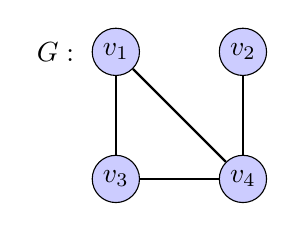
\begin{tikzpicture}[main node/.style={circle,fill=blue!20,draw,minimum size=.6cm,inner sep=0pt}]
    \node[main node] (1) {$v_1$};
    \node[main node] (2) [right = 1cm  of 1]  {$v_2$};
    \node[main node] (3) [below = 1cm  of 1] {$v_3$};
    \node[main node] (4) [right = 1cm  of 3] {$v_4$};
    \node[left = .1cm of 1]{$G:$};

    \path[draw,thick]
    (1) edge node {} (3)
    (1) edge node {} (4)
    (2) edge node {} (4)
    (3) edge node {} (4)
    ;
    \end{tikzpicture}
\caption{A visualisation of the simple graph $G =(V,E)$ with
$V=\{v_1,v_2,v_3,v_4\}$ and $E=\{(v_1,v_3), (v_1,v_4), (v_2,v_4), (v_3,v_4)\}$. }
\end{figure}
		
	}
\end{frame}

\begin{frame}[t]
	\frametitle{
		\LARGE{3. Graph colouring}}
			\visible<1->{\begin{definition}\label{vertex colouring}
A \textbf{vertex-colouring} of a graph $G=(V,E)$ is an assignment of colors from the set $\{1,...,k\}$ to $V$ such that each $v\in V$ is assigned one color and no two adjacent vertices are assigned the same color. 
\end{definition}}
%\todo{udkommenteret tikz}
%\iffalse
\visible<2->{
\begin{figure}[H]
\begin{tikzpicture}[main node/.style={circle,fill=blue!20,draw,minimum size=.6cm,inner sep=0pt}, scale =.8]
    \node[main node, fill = blue!60] (1) {$v_1$};
    \node[main node, fill = red!60] (2) [right = 1.1cm  of 1]  {$v_2$};
    \node[main node, fill = yellow!60] (3) [below left = .8cm and .6cm of 1] {$v_3$};
    \node[main node, fill = orange!60] (4) [below right = .8cm and .6cm of 2] {$v_4$};
    \node[main node, fill = purple!60] (5) [below = 2cm  of 1] {$v_5$};
    \node[main node, fill = green!60] (6) [right = 1.1cm  of 5] {$v_6$};
    \node[left = 1cm of 1]{$G:$};

    \path[draw,thick]
    (1) edge node {} (2)
    (1) edge node {} (3)
    (1) edge node {} (5)
    (2) edge node {} (3)
    (2) edge node {} (4)
    (2) edge node {} (5)
    (3) edge node {} (4)
    (3) edge node {} (6)
    (4) edge node {} (5)
    (5) edge node {} (6);
    %%
    }
    \visible<3->{
    \begin{scope}[xshift=6cm]
    \node[main node, fill = blue!60] (1) {$v_1$};
    \node[main node, fill = red!60] (2) [right = 1.1cm  of 1]  {$v_2$};
    \node[main node, fill = yellow!60] (3) [below left = .8cm and .6cm of 1] {$v_3$};
    \node[main node, fill = blue!60] (4) [below right = .8cm and .6cm of 2] {$v_4$};
    \node[main node, fill = yellow!60] (5) [below = 2cm  of 1] {$v_5$};
    \node[main node, fill = blue!60] (6) [right = 1.1cm  of 5] {$v_6$};
    \node[left = 1cm of 1]{$G:$};

    \path[draw,thick]
    (1) edge node {} (2)
    (1) edge node {} (3)
    (1) edge node {} (5)
    (2) edge node {} (3)
    (2) edge node {} (4)
    (2) edge node {} (5)
    (3) edge node {} (4)
    (3) edge node {} (6)
    (4) edge node {} (5)
    (5) edge node {} (6)
    ;
    \end{scope}
\end{tikzpicture}
\caption{A graph coloured with the trivial and an optimal vertex colouring.}
\end{figure}
}
\end{frame}


\begin{frame}[t]
\frametitle{
		\LARGE{3. Graph colouring}}
		\visible<1->{
		\begin{definition}\label{cromatic number}
The \textbf{chromatic number} $\chi (G)$ of a graph $G$ is the number of colours in an optimal colouring of $G$.
\end{definition}}
		\visible<2->{
		\begin{theorem}
	Given a graph $G$, with clique-number $\omega(G)$  $$|V| \geq \chi (G) \geq \omega(G).$$
	\end{theorem}
		}
		\visible<3->{
		Can we do this using linear programming?
		}
\end{frame}


\begin{frame}[t]
\frametitle{
		\LARGE{4. Integer programming}}
		\visible<2->{
		A way of formulating optimization problems with integer values.\\
		}
		\visible<3->{
					\begin{align*}
\begin{array}{ll@{}ll}
\text{min/max} &z(x_1,...,x_n)&\\
\text{s.t.} &g_1(x_1,...,x_n) \textbf{ ordRel } b_1,&\\
&\vdots&\\
&g_m(x_1,...,x_n) \textbf{ ordRel } b_m&\\
&\text{where each \textbf{ordRel} can be }\leq,\geq \text{ or } =&
\end{array}
					\end{align*}
			}
			\visible<4->{ $\exists x_i \in \{x_1,...,x_n\} : x_i \in \Z$\\}
			\visible<5->{These problems are hard to solve, but can solved in $\mathcal{NP}$-hard problems.}

\end{frame}

\begin{frame}[t]
\frametitle{
		\LARGE{4. Integer programming}}
		The feasible set and optimal solutions
		\visible<2->{
		\begin{figure}[H]
\centering
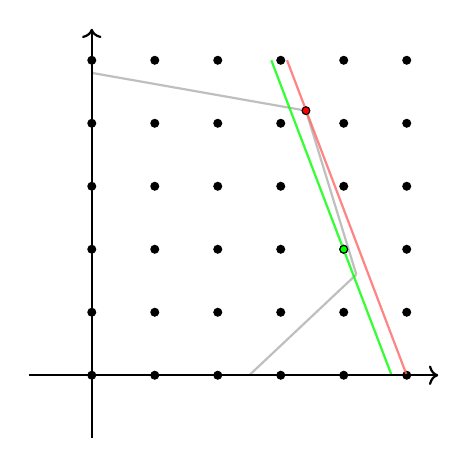
\begin{tikzpicture}[scale = 0.8]
\foreach \x in {0,...,5}{
	\foreach \y in {0,...,5}{% node on the grid we have drawn 
        \node[draw,circle,inner sep=1pt,fill] at (\x,\y) {};
            % Places a dot at those points
  }
}
\draw [lightgray, thick] (0,4.8) -- (3.4,4.2);
\draw [lightgray, thick] (3.4,4.2)--(4.2,1.6);
\draw [lightgray, thick] (4.2,1.6)--(2.5,0);
\draw [red!60,opacity=.8, thick] (3.1,5)--(5,0);
\node[draw,circle,inner sep=1pt,fill = red] at (3.4,4.2) {};
\draw [green,opacity=.8, thick] (2.85,5)--(4.76,0);
\node[draw,circle,inner sep=1pt,fill = green] at (4,2) {};
\draw [black, thick, arrows = ->] (0,-1) -- (0,5.5);
\draw [black, thick, arrows = ->] (-1,0) -- (5.5,0);
\end{tikzpicture}
\caption{Figure showing the feasible region of an IP with the optimal solution in green and the optimal solution to the linear relaxation in red.}
\end{figure}
		}
\end{frame}


\begin{frame}[t]
\frametitle{
		\LARGE{4. Integer programming}}
		Using MIP to solve problems in graph theory
		\visible<2->{
\begin{figure}[H]
\centering
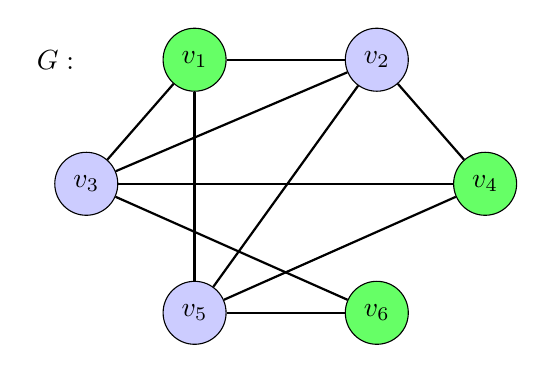
\begin{tikzpicture}[main node/.style={circle,fill=blue!20,draw,minimum size=.8cm,inner sep=0pt}]
    \node[main node,fill = green!60] (1) {$v_1$};
    \node[main node] (2) [right = 1.5cm  of 1]  {$v_2$};
    \node[main node] (3) [below left = 1cm and .8cm of 1] {$v_3$};
    \node[main node,fill = green!60] (4) [below right = 1cm and .8cm of 2] {$v_4$};
    \node[main node] (5) [below = 2.4cm  of 1] {$v_5$};
    \node[main node,fill = green!60] (6) [right = 1.5cm  of 5] {$v_6$};
    \node[left = 1cm of 1]{$G:$};

    \path[draw,thick]
    (1) edge node {} (2)
    (1) edge node {} (3)
    (1) edge node {} (5)
    (2) edge node {} (3)
    (2) edge node {} (4)
    (2) edge node {} (5)
    (3) edge node {} (4)
    (3) edge node {} (6)
    (4) edge node {} (5)
    (5) edge node {} (6)
    ;
    \end{tikzpicture}
\caption{Shown in green is a maximum independent set in a graph $G$.}
\end{figure}
}
\visible<3->{
\vspace*{-.6cm}
\begin{align*}
\begin{array}{ll@{}ll}
\text{max} &\sum_{v\in V} x_v&\\
\text{s.t.} &x_u + x_v \leq 1,& \forall (u,v) \in E\\
&x_v\in\{0,1\},& \forall v \in V\\
\end{array}
\end{align*}

		}
\end{frame}

\begin{frame}[t]
\frametitle{
		\LARGE{4. Integer programming}}
		Some strategies used in integer programming
		\begin{enumerate}
		\item<2-> Big-M strategy, creating a constraint $x_1 \neq x_2$
			\begin{enumerate}
			\item[]<3-> For $x_1,x_2 \in \Z ,$ $ t \in \{0,1\}$ and suitable large $M$, two constraints
			 \begin{align*}
x_1-x_2 + Mt \leq M-1\\
\text{and}\\
x_2-x_1 - Mt \leq -1
\end{align*}
ensures that no feasible solution has $x_1 = x_2$.
			\end{enumerate}
		\item<4-> A strategy for determining the difference $|x_1 - x_2|$ of binary variables
			\begin{enumerate}
			\item[]<5-> For $x_1,x_2,z,t \in \{0,1\}$, the constraint
			\begin{align*}
			x_1-x_2 - 2t + z = 0
			\end{align*}
			Ensures that in a feasible solution, $z = |x_1 - x_2|$
			\end{enumerate}
		\end{enumerate}
\end{frame}

\begin{frame}[t]
\frametitle{
		\LARGE{5. IP colouring formulations}}
		\visible<2->{
		\large{The standard formulation\\}
		}
		\visible<3->{
		For any $k \geq \chi(G)$
\begin{align*}
\begin{array}{ll@{}ll}
\text{min} &\sum_{c\in \{1...k\}} y_c&\\
\text{s.t.} 
&\sum_{c\in \{1...k\}}{x_{v,c}} = 1, \quad & \forall v \in V\\
&x_{v,c} + x_{u,c} \leq 1,& \forall (u,v)\in E, \, \forall c \in \{1...k\}\\
&x_{v,c} - y_c \leq 0,& \forall v \in V, \,\forall c \in \{1...k\}\\
&x_{v,c}\in\{0,1\},& \forall v \in V, \, \forall c \in \{1...k\}\\
&y_c \geq 0,& \forall c \in \{1...k\}\\
\end{array}
\end{align*}
$k|V|+k$ binary variables and $|V|+k|E|+k|V|$ constraints.
		}
\end{frame}

\begin{frame}[t]
\frametitle{
		\LARGE{5. IP colouring formulations}}	
				\visible<1->{
		\large{The scheduling formulation\\}
		}
		\visible<2->{
		For any $k \geq \chi(G)$
		\begin{align*}
\begin{array}{ll@{}ll}
\text{min} &c&\\
\text{s.t.} 
&X_u - X_v + kx_{u,v} \leq k-1, \quad & \forall (u,v)\in E\\
&X_v - X_u - kx_{u,v} \leq -1,& \forall (u,v)\in E\\
&X_v - c \leq 0,& \forall v \in V\\
&x_{u,v}\in\{0,1\},& \forall (u,v) \in E\\
\end{array}
\end{align*}
$|V|+|E|$ integer and binary variables and $2|E|+|V|$ constraints.
		}
\end{frame}

\begin{frame}[t]
\frametitle{
		\LARGE{5. IP colouring formulations}}
						\visible<1->{
		\large{The binary formulation\\}
		}
		\visible<2->{
		For any $k \geq \chi(G)$, suppose $B = \left \lceil{log_2(k)}\right \rceil$:
		\begin{align*}
\begin{array}{ll@{}ll}
\text{min} &c&\\
\text{s.t.} 
&c - \sum_{b = 0}^{B}{2^b\cdot x_{v,b}} \leq -1,& \forall v\in V\\
&z_{v,u,b}-2t_{v,u,b}+x_{v,b}-x_{u,b} = 0,\quad & \forall (u,v)\in E \, \forall \, b \in [0,\cdots ,B ] \\
&\sum_{b = 0}^{B}{z_{v,u,b}} \geq 1,& \forall (u,v) \in E\\
&x_{v,b}\in\{0,1\},& \: \forall \, v \in V \, \forall \, b \in [0,\cdots ,B]\\
&z_{u,v,b}\in\{0,1\},& \forall (u,v) \in E \: \forall \, b \in [0,\cdots ,B]\\
&x_{u,v,b}\in\{0,1\},& \forall (u,v) \in E \: \forall \, b \in [0,\cdots ,B]\\
\end{array}
\end{align*}
\noindent $|V|\left \lceil{log_2(k)}\right \rceil + 2|E|\left \lceil{log_2(k)}\right \rceil$ binary variables and $|V|+|E|+|E|\left \lceil{log_2(k)}\right \rceil$ constraints.
		}
\end{frame}

\begin{frame}[t]
\frametitle{
		\LARGE{5. IP colouring formulations}}
		Industrial MIP solvers
		
		
		\visible<2->{CPLEX}
		\visible<3->{
		\begin{figure}
		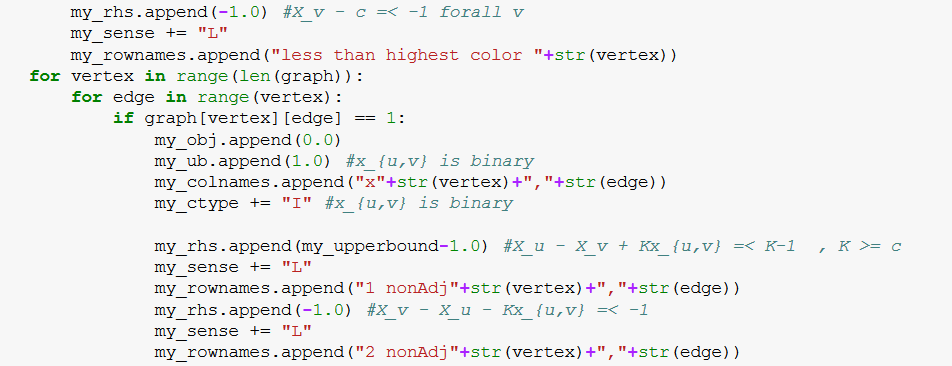
\includegraphics[scale=.55]{schedul.PNG}
		\caption{A section of my code implementing the scheduling formulation using the CPLEX Python-API.}
		\end{figure}
		}
\end{frame}

\begin{frame}[t]
\frametitle{
		\LARGE{6. Lego graphs}}
		\visible<2->{Colouring $a\times b$-brick Lego buildings\\}
		\visible<3->{Constructing graphs to find an upper bound on their chromatic number}
		\visible<4->{
		\begin{figure}
		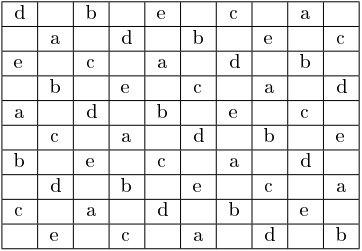
\includegraphics[scale=.9]{12gprime.PNG}
		\caption{The method for finding upper bounds on colours $1\times 2$-brick buildings as developed by AHBS.}
		\end{figure}
		}
\end{frame}

\begin{frame}[t]
\frametitle{
		\LARGE{6. Lego graphs}}
		\visible<1->{Colouring $a\times b$-brick Lego buildings\\}
		\visible<1->{Constructing graphs to find an upper bound on their chromatic number}
		\visible<1->{
		\begin{figure}
		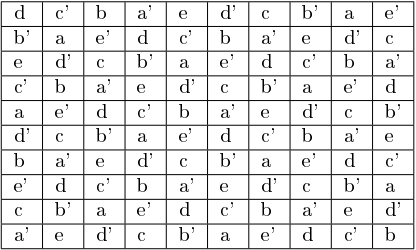
\includegraphics[scale=.9]{12g.PNG}
		\caption{The method for finding upper bounds on colours $1\times 2$-brick buildings as developed by AHBS.}
		\end{figure}
		}
\end{frame}

\begin{frame}[t]
\frametitle{
		\LARGE{6. Lego graphs}}
		\visible<2->{$G[a,b;c,d]$ Lego graphs:\\}
		\visible<3->{
		A vertex at every possible position of a brick.\\
		}
		\visible<4->{
		$2cd$ vertices for $a=b$ and $4cd$ vertices for $a \neq b$.\\
		}
		\visible<5->{ An edge if two bricks or their periodic translates touch.
		}
		\visible<6->{
				\begin{figure}
\centering
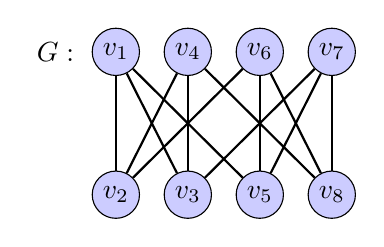
\begin{tikzpicture}[main node/.style={circle,fill=blue!20,draw,minimum size=.6cm,inner sep=0pt}]
    \node[main node] (1) {$v_1$};
    \node[main node] (2) [below = 1.2cm  of 1]  {$v_2$};
    \node[main node] (3) [right = .3cm  of 2] {$v_3$};
    \node[main node] (4) [right = .3cm  of 1] {$v_4$};
    \node[main node] (5) [right = .3cm  of 3]{$v_5$};
    \node[main node] (6) [right = .3cm  of 4]  {$v_6$};
    \node[main node] (7) [right = .3cm  of 6] {$v_7$};
    \node[main node] (8) [right = .3cm  of 5] {$v_8$};
    \node[left = .1cm of 1]{$G:$};

    \path[draw,thick]
    (1) edge node {} (2)
    (1) edge node {} (3)
    (1) edge node {} (5)
    (2) edge node {} (4)
    (2) edge node {} (6)
    (3) edge node {} (4)
    (3) edge node {} (7)
    (4) edge node {} (8)
    (5) edge node {} (6)
    (5) edge node {} (7)
    (6) edge node {} (8)
    (7) edge node {} (8)
    ;
    \end{tikzpicture}
\caption{The graph $G[1,1;2,2]$. }
		\end{figure}
		}
\end{frame}

\begin{frame}[t]
\frametitle{
		\LARGE{7. Exciting results}}
		\visible<2->{A comparison of the different formulations}
		\visible<3->{
		\scriptsize	
		\begin{table}
		\centering	
		\begin{tabular}{|lll|lll|lll|lll|}
		\hline
\multicolumn{3}{|c|}{Graph}&\multicolumn{3}{c|}{Standard}&\multicolumn{3}{c|}{Scheduling} &\multicolumn{3}{c|}{Binary}\\
Name&$|V|$&$k$&lb&ub&time&lb&ub&time&lb&ub&time\\
\hline
miles1000&128&44&42&42&2s&4&43&30.0m&?&?&30.0m\\
\hline
miles1500&128&73&73&73&21s&4&73&30.0m&?&?&30.0m\\
\hline
miles250&128&9&8&8&0s&8&8&55s&?&?&30.0m\\
\hline
miles500&128&21&20&20&0s&5&20&30.0m&?&?&30.0m\\
\hline
miles750&128&32&31&31&1s&4&31&30.0m&?&?&30.0m\\
\hline
myciel3&11&4&4&4&0s&4&4&0s&4&4&0s\\
\hline
myciel4&23&5&5&5&0s&5&5&0s&5&5&22s\\
\hline
myciel5&47&6&6&6&22s&5&6&30.0m&4&6&30.0m\\
\hline
myciel6&95&7&5&7&30.0m&4&7&30.0m&3&7&30.0m\\
\hline
myciel7&191&8&4&8&30.0m&4&8&30.0m&3&8&30.0m\\
\hline
Q\_10\_4\_3&120&21&8&17&30.0m&4&18&30.0m&?&?&30.0m\\
\hline
Q\_10\_4\_5&252&30&7&27&30.0m&3&30&30.0m&?&?&30.0m\\
\hline
Q\_7\_4&64&9&8&8&0s&5&8&30.0m&?&?&30.0m\\
\hline
Q\_8\_2&128&15&8&8&1s&5&8&30.0m&?&?&30.0m\\
\hline
Q\_8\_4&128&9&8&8&7s&5&8&30.0m&?&?&30.0m\\
\hline
Q\_9\_2&256&19&9&16&30.0m&3&18&30.0m&?&?&30.4m\\
\hline
		\end{tabular}
		\caption{A section of the colouring results}
		\end{table}
		}
\end{frame}

\begin{frame}[t]
\frametitle{
		\LARGE{7. Exciting results}}
		\visible<1->{A comparison of the different formulations}
		\begin{itemize}
		\item<2-> Proven optimal solutions within 30 minutes:
		\begin{itemize}
		\item<3-> The standard formulation: $62\%$ of the test-set
		\item<4-> The scheduling formulation: $41\%$ of the test-set
		\item<5-> The binary formulation: $19\%$ of the test-set
		\end{itemize}
		\item<6-> The scheduling formulations found optimal upper bounds, but struggled to prove the lower bounds. 
		\item<7-> The binary formulation struggled to find any integer solutions at all.
		\item<8-> The standard formulation was fastest in most cases, but the scheduling formulation was better in some of the Lego graphs.
		\end{itemize}
\end{frame}

\begin{frame}[t]
\frametitle{
		\LARGE{7. Exciting results}}
		Lego graph results
		\visible<2->{
		\scriptsize	
		\begin{table}
		\centering	
		\begin{tabular}{|lll|lll|lll|lll|}
		\hline
\multicolumn{3}{|c|}{Graph}&\multicolumn{3}{c|}{Standard}&\multicolumn{3}{c|}{Scheduling} &\multicolumn{3}{c|}{Binary}\\
Name&$|V|$&$k$&lb&ub&time&lb&ub&time&lb&ub&time\\
\hline
G\_1\_2\_10\_10&400&11&5&5&16.2m&5&5&57s&?&?&30.3m\\
\hline
G\_2\_2\_6\_6&72&8&5&5&2s&5&5&1s&5&5&36s\\
\hline
G\_3\_3\_10\_10&200&12&6&7&30.0m&4&7&30.0m&?&?&30.0m\\
\hline
\end{tabular}
		\caption{The best upper bounds found for $1\times 2$,$2\times 2$ and $3\times 3$ brick buildings.}
		\end{table}
		}
		\visible<3->{
		\begin{table}
\centering
\begin{tabular}{|lll|lll|lll|}
\hline
\multicolumn{3}{|c|}{Graph}&\multicolumn{3}{c|}{Standard}&\multicolumn{3}{c|}{Scheduling}\\
Name&$|V|$&$k$&lb&ub&time&lb&ub&time\\
\hline
G\_1\_2\_10\_12&480&4&5&?&1.9m&5&?&1.4m\\
\hline  
G\_1\_2\_12\_12&576&4&5&?&5.7m&5&?&2.6m\\
\hline
G\_3\_3\_10\_10&200&6&7&?&20.9m&?&?&30.0m\\
\hline
G\_3\_3\_12\_12&288&6&7&?&1.5h&\multicolumn{3}{c}{}\\
\cline{1-6}
\end{tabular}
\caption{Results from trying to find 4-colourable $1 \times 2$, and 6-colourable $3\times 3$ Lego graphs.}
\end{table}
}
\end{frame}

\begin{frame}[t]
\frametitle{
		\LARGE{8. Short summary}}
		\begin{itemize}
		\item<2-> Graph colouring is very useful for many different purposes.
		\item<3-> Mathematical optimization can be used for colouring graphs, but linear programming is not enough.
		\item<4-> Different IP formulations perform better or worse depending on the graph, but no clear picture of when one outperforms another is visible. 
		\item<5-> No ground breaking new results have been found for colouring Lego buildings, but IP seems to be an efficient approach to finding such results.
		\item[]<6-> \vspace*{1cm} \begin{center} Thank you for listening.\end{center}
		\end{itemize}
\end{frame}

\begin{frame}[c]{}
		\centering
		\Huge{Questions}
\end{frame}


\end{document}